\begingroup
\setstretch{1}
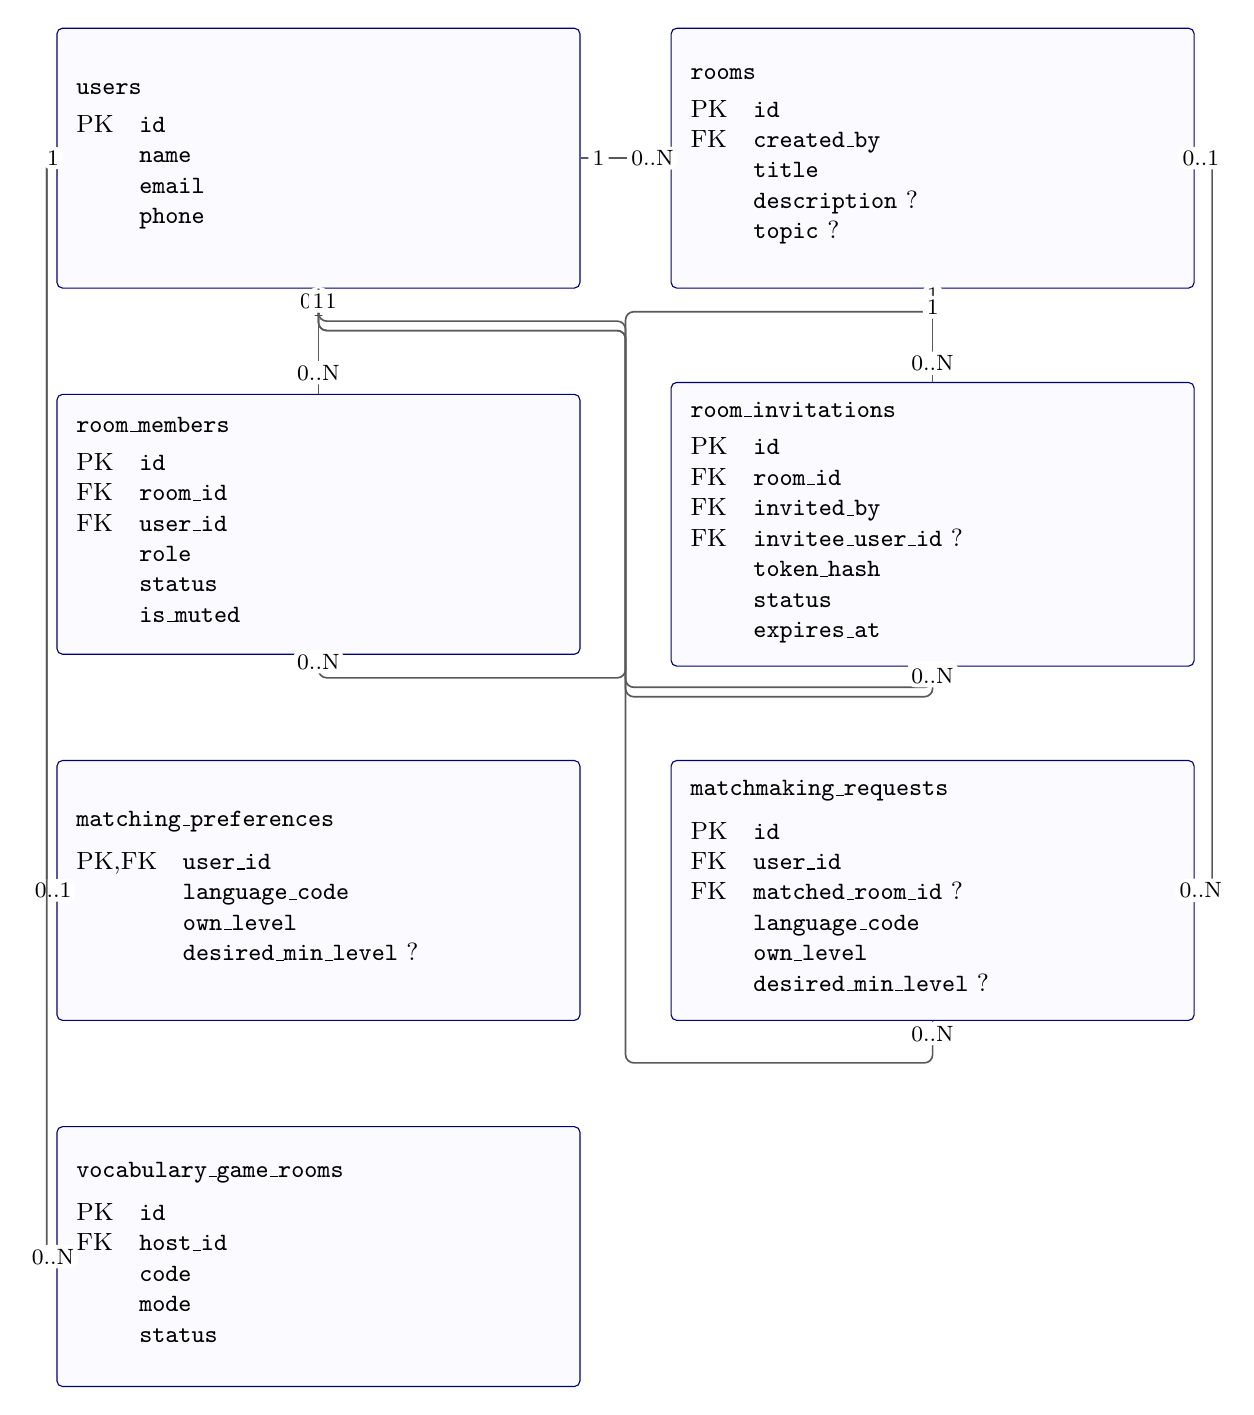
\begin{tikzpicture}[
entity/.style={draw=blue!45!black,rounded corners=2pt,fill=blue!2,inner sep=7pt,text width=6.15cm,minimum height=3.3cm,align=left,font=\fontsize{9}{11}\selectfont},
rel/.style={draw=black!65,line width=.6pt,rounded corners=3pt},
card/.style={fill=white,inner sep=1.5pt,font=\fontsize{8}{9}\selectfont}]
\node[entity] (users) at (-3.9,0) {\textbf{\texttt{users}}\\[5pt]\begin{tabular}{@{}l@{\quad}l@{}}PK & \texttt{id} \\
 & \texttt{name} \\
 & \texttt{email} \\
 & \texttt{phone} \\\end{tabular}};
\node[entity] (rooms) at (3.9,0) {\textbf{\texttt{rooms}}\\[5pt]\begin{tabular}{@{}l@{\quad}l@{}}PK & \texttt{id} \\
FK & \texttt{created\_by} \\
 & \texttt{title} \\
 & \texttt{description} ? \\
 & \texttt{topic} ? \\\end{tabular}};
\node[entity] (roommembers) at (-3.9,-4.65) {\textbf{\texttt{room\_members}}\\[5pt]\begin{tabular}{@{}l@{\quad}l@{}}PK & \texttt{id} \\
FK & \texttt{room\_id} \\
FK & \texttt{user\_id} \\
 & \texttt{role} \\
 & \texttt{status} \\
 & \texttt{is\_muted} \\\end{tabular}};
\node[entity] (roominvitations) at (3.9,-4.65) {\textbf{\texttt{room\_invitations}}\\[5pt]\begin{tabular}{@{}l@{\quad}l@{}}PK & \texttt{id} \\
FK & \texttt{room\_id} \\
FK & \texttt{invited\_by} \\
FK & \texttt{invitee\_user\_id} ? \\
 & \texttt{token\_hash} \\
 & \texttt{status} \\
 & \texttt{expires\_at} \\\end{tabular}};
\node[entity] (matchingpreferences) at (-3.9,-9.3) {\textbf{\texttt{matching\_preferences}}\\[5pt]\begin{tabular}{@{}l@{\quad}l@{}}PK,FK & \texttt{user\_id} \\
 & \texttt{language\_code} \\
 & \texttt{own\_level} \\
 & \texttt{desired\_min\_level} ? \\\end{tabular}};
\node[entity] (matchmakingrequests) at (3.9,-9.3) {\textbf{\texttt{matchmaking\_requests}}\\[5pt]\begin{tabular}{@{}l@{\quad}l@{}}PK & \texttt{id} \\
FK & \texttt{user\_id} \\
FK & \texttt{matched\_room\_id} ? \\
 & \texttt{language\_code} \\
 & \texttt{own\_level} \\
 & \texttt{desired\_min\_level} ? \\\end{tabular}};
\node[entity] (vocabularygamerooms) at (-3.9,-13.950000000000001) {\textbf{\texttt{vocabulary\_game\_rooms}}\\[5pt]\begin{tabular}{@{}l@{\quad}l@{}}PK & \texttt{id} \\
FK & \texttt{host\_id} \\
 & \texttt{code} \\
 & \texttt{mode} \\
 & \texttt{status} \\\end{tabular}};
\draw[rel] (rooms.west) -- node[card,pos=.2]{0..N} node[card,pos=.8]{1} (users.east);
\draw[rel] (roommembers.south) -- node[card,pos=.3]{0..N} (-3.9,-6.6000000000000005) -- (0,-6.6000000000000005) -- (0,-1.95) -- (3.9,-1.95) -- node[card,pos=.7]{1} (rooms.south);
\draw[rel] (roommembers.north) -- node[card,pos=.2]{0..N} node[card,pos=.8]{1} (users.south);
\draw[rel] (roominvitations.south) -- node[card,pos=.3]{0..N} (3.9,-6.720000000000001) -- (0,-6.720000000000001) -- (0,-2.07) -- (-3.9,-2.07) -- node[card,pos=.7]{1} (users.south);
\draw[rel] (roominvitations.south) -- node[card,pos=.3]{0..N} (3.9,-6.840000000000001) -- (0,-6.840000000000001) -- (0,-2.19) -- (-3.9,-2.19) -- node[card,pos=.7]{0..1} (users.south);
\draw[rel] (roominvitations.north) -- node[card,pos=.2]{0..N} node[card,pos=.8]{1} (rooms.south);
\draw[rel] (matchingpreferences.west) -- node[card,pos=.35]{0..1} (-7.35,-9.3) -- (-7.35,0) -- node[card,pos=.65]{1} (users.west);
\draw[rel] (matchmakingrequests.east) -- node[card,pos=.35]{0..N} (7.449999999999999,-9.3) -- (7.449999999999999,0) -- node[card,pos=.65]{0..1} (rooms.east);
\draw[rel] (matchmakingrequests.south) -- node[card,pos=.3]{0..N} (3.9,-11.49) -- (0,-11.49) -- (0,-2.19) -- (-3.9,-2.19) -- node[card,pos=.7]{1} (users.south);
\draw[rel] (vocabularygamerooms.west) -- node[card,pos=.35]{0..N} (-7.35,-13.950000000000001) -- (-7.35,0) -- node[card,pos=.65]{1} (users.west);
\end{tikzpicture}
\endgroup
